\section{Ход работы}
\subsection{Измерения}

1. Измерен перепад высоты столбика ртути на U-образном манометре с помощью микорокопа и температура по индикаторному табло. Результаты приведены в таблице \ref*{table:vverh}.

2. Проведены измерения, аналогичные измерениям в 1 пункте при нагревании термостата, как следствие, нагревании воды (исследуемой жидкости). Результаты приведены в таблице \ref*{table:vverh}.

\begin{table}[ht]
    \centering
    \begin{tabular}{|c|c|c|c|c|}
        \hline
        h1, см & h2, см & $\Delta h$, см & $P$, Па & T, $\text{}^\circ C$\\
        \hline
        7,19 & 8,87 & 1,68 & 2241,3888 & 23,06 \\
		\hline
		7,12 & 8,88 & 1,76 & 2348,1216 & 24,09 \\
		\hline
		7,07 & 8,94 & 1,87 & 2494,8792 & 25,07 \\
		\hline
		6,99 & 9,045 & 2,055 & 2741,6988 & 26,08 \\
		\hline
		6,92 & 9,125 & 2,205 & 2941,8228 & 27,08 \\
		\hline
		6,85 & 9,235 & 2,385 & 3181,9716 & 28,07 \\
		\hline
		6,76 & 9,32 & 2,56 & 3415,4496 & 29,08 \\
		\hline
		6,69 & 9,435 & 2,745 & 3662,2692 & 30,07 \\
		\hline
		6,61 & 9,51 & 2,9 & 3869,064 & 31,07 \\
		\hline
		6,53 & 9,64 & 3,11 & 4149,2376 & 32,09 \\
		\hline
		6,46 & 9,73 & 3,27 & 4362,7032 & 33,08 \\
		\hline
		6,37 & 9,84 & 3,47 & 4629,5352 & 34,09 \\
		\hline
		6,25 & 9,95 & 3,7 & 4936,392 & 35,07 \\
		\hline
		6,115 & 10,09 & 3,975 & 5303,286 & 36,06 \\
		\hline
		6,025 & 10,2 & 4,175 & 5570,118 & 37,05 \\
		\hline
		5,9 & 10,365 & 4,465 & 5957,0244 & 38,04 \\
		\hline
    \end{tabular}
    \caption{Зависимость давления насященного пара от температуры при увеличении температуры}
    \label{table:vverh}
\end{table}

3. Проведены аналогичные измерения пунктам 1 и 2, но при уменьшении температуры. Результаты приведены в таблице \ref*{table:vniz}.
\begin{table}[ht]
    \centering
    \begin{tabular}{|c|c|c|c|c|}
        \hline
        h1, см & h2, см & $\Delta h$, см & $P$, Па & T, $\text{}^\circ C$\\
        \hline
		5,8 & 10,48 & 4,68 & 6243,8688 & 38,04 \\
		\hline
		5,92 & 10,32 & 4,4 & 5870,304 & 36,77 \\
		\hline
		6,13 & 10,11 & 3,98 & 5309,9568 & 35,04 \\
		\hline
		6,34 & 9,86 & 3,52 & 4696,2432 & 33,04 \\
		\hline
		5,83 & 8,97 & 3,14 & 4189,2624 & 31,06 \\
		\hline
		6 & 8,76 & 2,76 & 3682,2816 & 29,04 \\
		\hline
		6,195 & 8,61 & 2,415 & 3221,9964 & 27,05 \\
		\hline
		6,33 & 8,4 & 2,07 & 2761,7112 & 25,07 \\
		\hline
    \end{tabular}
    \caption{Зависимость давления насященного пара от температуры при понижении температуры}
    \label{table:vniz}
\end{table}

\subsection{Обработка}

4. Построены графики $P(T)$ и $\ln{P}(\frac 1 T)$:

\begin{minipage}{\linewidth}
	\centering
	\begin{minipage}{0.45\linewidth}
		\begin{figure}[H]
			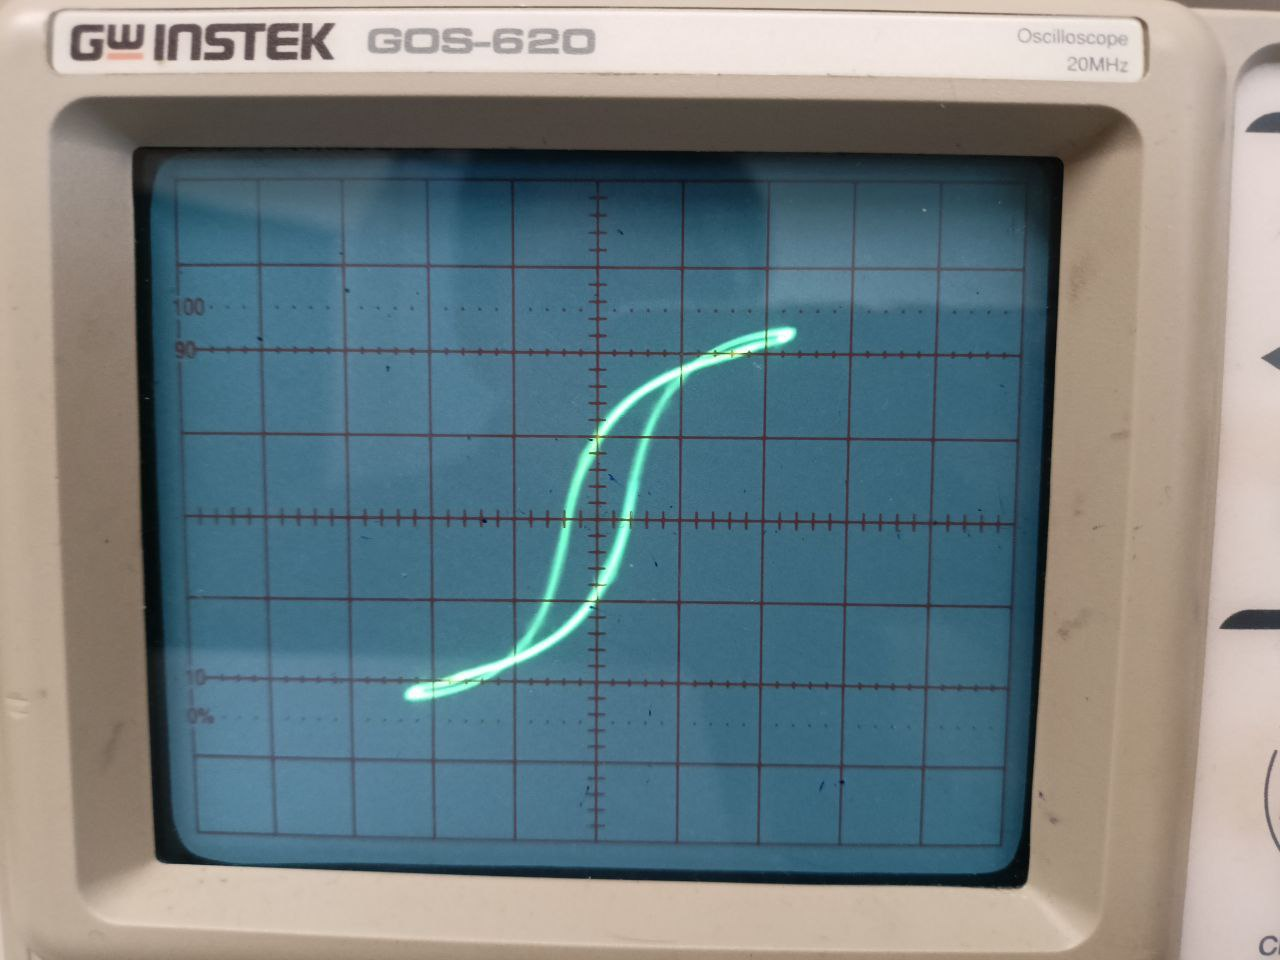
\includegraphics[width=\linewidth]{p1.jpg}
		\end{figure}
	\end{minipage}
	\hspace{0\linewidth}
	\begin{minipage}{0.45\linewidth}
		\begin{figure}[H]
			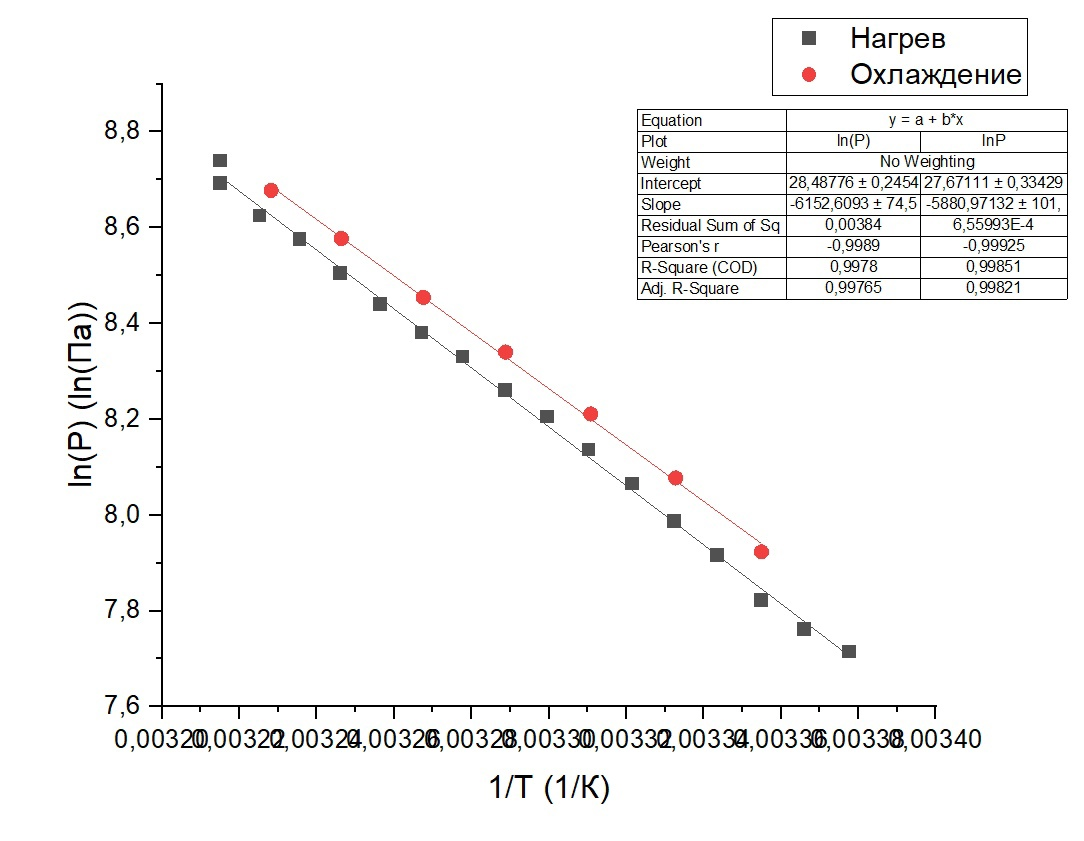
\includegraphics[width=\linewidth]{p2.jpg}
		\end{figure}
	\end{minipage}
\end{minipage}


5. В случае нагревания $\frac{d\left(\ln(P)\right)}{d\left(\frac 1 T\right)} = -6152 \pm 80$, а в случае охлаждения $\frac{d\left(\ln(P)\right)}{d\left(\frac 1 T\right)} = -5889 \pm 100$.
Посчитаем для каждого из случае теплоту испарения жидкости:
\[L_\text{нагр} = (51128 \pm 600) \text{ } \frac{\text{Дж}}{\text{моль}},\]
\[L_\text{охл} = (48871 \pm 800) \text{ }\text{ } \frac{\text{Дж}}{\text{моль}}.\]

6. Чтобы получить значения для удельной теплоты испарения, необходимо разделить на молярную массу воды $\mu = 18 \text{ г} / \text{моль}$:
\[q_\text{нагр} = (28,4 \pm 0,4) \cdot 10^5 \text{ } \frac{\text{Дж}}{\text{кг}},\]
\[q_\text{охл} = (27,2 \pm 0,5) \cdot 10^5 \text{ } \frac{\text{Дж}}{\text{кг}}.\]
